%!TEX root = ../template.tex
%%%%%%%%%%%%%%%%%%%%%%%%%%%%%%%%%%%%%%%%%%%%%%%%%%%%%%%%%%%%%%%%%%%%
%% chapter4.tex
%% NOVA thesis document file
%%
%% Chapter with lots of dummy text
%%%%%%%%%%%%%%%%%%%%%%%%%%%%%%%%%%%%%%%%%%%%%%%%%%%%%%%%%%%%%%%%%%%%
\chapter{State of the Art}
\label{cha:SotA}


\section{Social Networks}
\label{sec:SocialNet}

%Beggining of Social Network Analysis
\par
Social Network Theory and Analysis, these are the area that study the currently emerging networks. \\
Network communication can be found all around us human bodies have them (Neves et al, 2008), physics, politics, computer science, etc. Socially, in later years, networks have been developed used many important websites like facebook, twitter, Instagram. This has created a new importunity for marketing and analysis. 
Since this work is mainly focused on feedback I’ll focus more on that particular area.

\par
Before defining different network types it's important to connect common definitions to social networks language.

\begin{itemize}
	\item Nodes: In this case can be associated with Authors or Posts, may apply to a specific person or a post on social media depending if we are evaluating user network or posts networks
	
	\item Relations: This defines the tie between authors or posts. Ties where both nodes are related in the same way (eg. Two different authors commented on same post) are called undirected.
	
	\par Relationship when relation is different on both ends are considered directed. These connections can be one directional, an authors replying to a post from another author, or bi directional the reply to a post.
	
	\item Weighted Relations: Not all tie are alike, some nodes may have stronger connections while others might have a smaller impact between each other
	 
	\item Network: The collection of authors and ties. When multiple networks are created and overlapped it becomes a Multiplex network. This evolved state is present in many social media, creating multiple and different relations between authors.
	
\end{itemize} 

%Create Node Image Showing a Centralized network, Decentralized and Distributed

\begin{figure}[htbp]
	\centering
	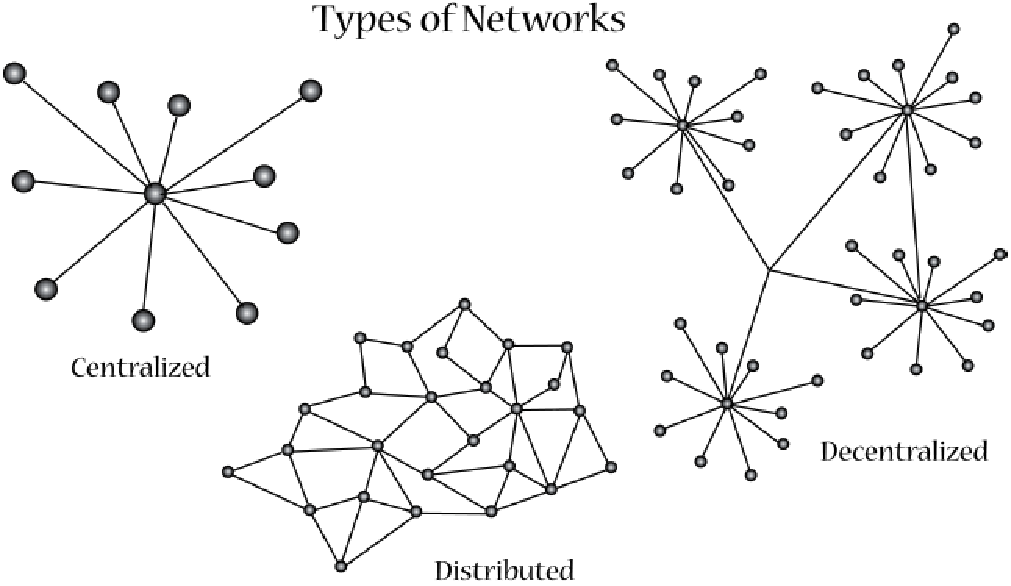
\includegraphics[height=2in]{network-types-pdf}
	\caption{Network Types}
	\label{fig:NetworkTypesImg}
\end{figure}

Figure \ref{fig:NetworkTypesImg} shows some examples of network diagrams. Centralized networks are highly advantageous  connection wise, everyone can give information to each other within 2 step, but fail when the centralized node is offline for some reason, this stops the entire network.
\par
Before internet, companies had to rely on Decentralized networks to gather feedback, some still do. By decentralizing, the amount of nodes that fail when the upper node disappear is lower, although it still happens. The big advantage of this layout is that it can easily become a Distributed network. Outer and lower connection nodes can easily connect to each other and create redundancy. 
\begin{figure}[htbp]
	\centering
	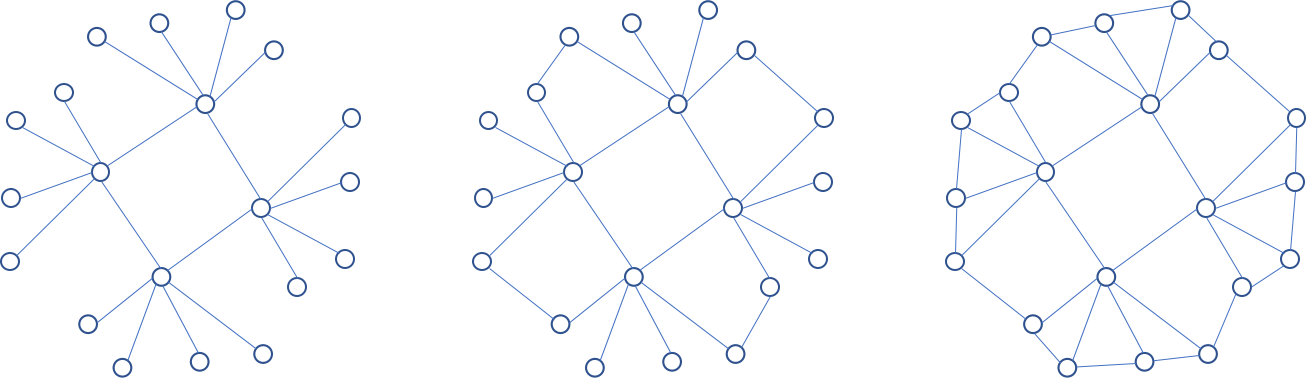
\includegraphics[width=\textwidth]{Decent-Distri}
	\caption{Decentralized to Distributed}
	\label{fig:Decent-Distri}
\end{figure}

\par
Distributed networks, occur when initially isolated nodes start to make connections with other nodes, something like in facebook when a user starts adding friends-of-friends, or following a page instead of waiting for a friend to share information from said page Figure \ref{fig:Decent-Distri}. This means that everyone has the same, or really close, importance in the network.A Layout like this is extremely utopic when thinking about feedback analysis. 
\par
While everyone has their own, valid, opinion on a product, people like celebrities can spread their opinion faster than a kindergartner. Realistically, decentralized networks are the most common occurrence.
\par



%End of Social Network Analysis

%Beggining of Natural Language Processing

\section{Natural Language Processing}
\par 



%End of Natural Language Processing
